\section{Ferramentas para testes de cobertura}
Dentre as várias opções de ferramentas para realizar testes de cobertura, foram escolhidas duas: \textbf{Hansel} e \textbf{Atlassian Clover}.
\begin{itemize}
    \item \textbf{Hansel:} Trata-se de uma extensão para \textit{JUnit} que possibilita a geração de testes de cobertura.
    \item \textbf{Atlassian Clover:} Possui integração com \textit{Eclipse} e também possibilita a geração de testes de cobertura.
\end{itemize}
A instalação do \textit{plugin Clover} para o \textit{Eclipse} foi bem fácil de resolver, bastou apenas adicionar novo software. No entanto, por alguma razão, embora fosse possível executar "\textit{Run Clover as $>>$ Run With Clover Configurations}", como ilustrado na figura \ref{figura:clover_configurations}, não foi possível gerar o relatório de cobertura.
Provavelmente causado por alguma configuração que deveria ter sido realizada em "\textit{Run with Clover configurations}", mostrada nas figuras \ref{figura:clover_junit} e \ref{figura:clover_coverage}.

\begin{figure}[H]
    \caption{\textit{Clover configurations}}
    \vspace{0.5cm}
    \centering
    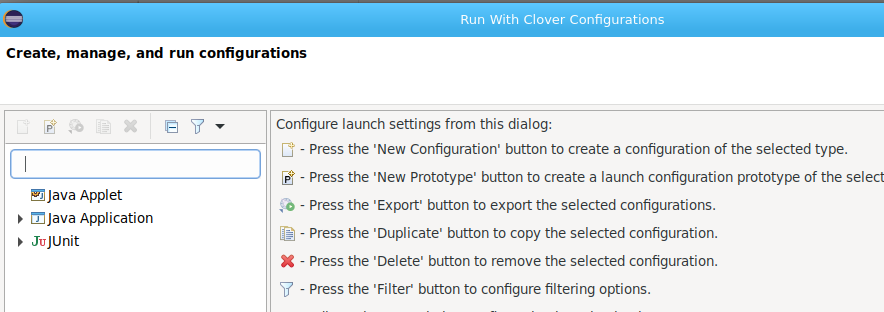
\includegraphics[width=15cm]{imagens/clover_configurations.png}
    \label{figura:clover_configurations}
\end{figure}

\begin{figure}[H]
    \caption{Página dos testes de cobertura}
    \vspace{0.5cm}
    \centering
    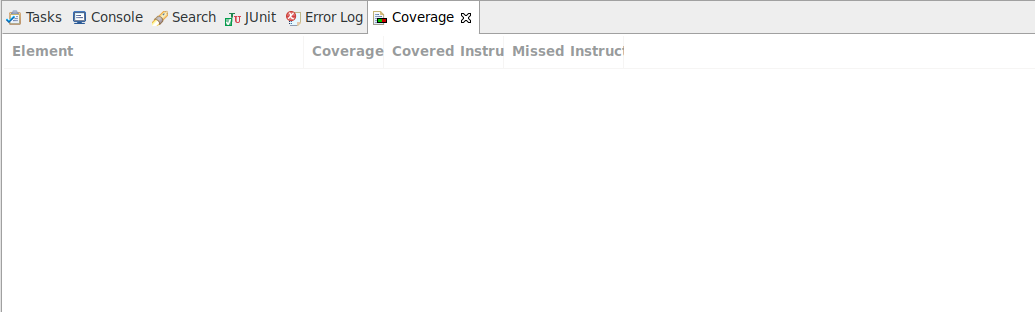
\includegraphics[width=15cm]{imagens/clover_coverage.png}
    \label{figura:clover_coverage}
\end{figure}

\begin{figure}[H]
    \caption{Página dos testes do \textit{JUnit}}
    \vspace{0.5cm}
    \centering
    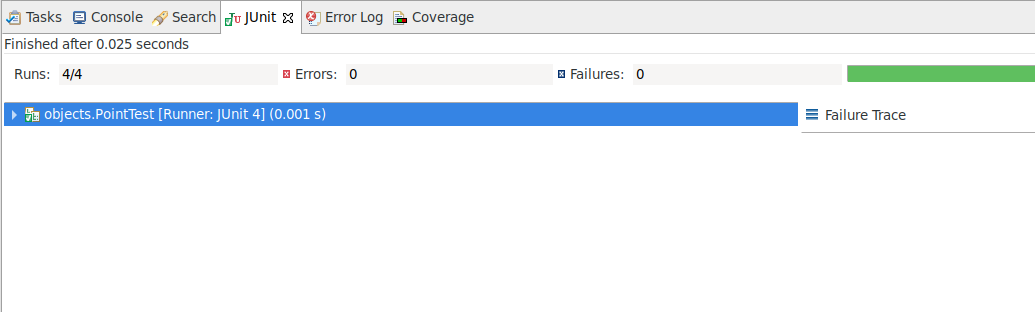
\includegraphics[width=15cm]{imagens/clover_junit.png}
    \label{figura:clover_junit}
\end{figure}

A instalação do \textit{Hansel}, por sua vez, não foi possível resolver, talvez esteja relacionado a um link de instalação obsoleto. Poucos foram os links encontrados para solução de problemas desse tipo.
